% begin Chapter LiteratureReview

\chapter {Literature Review}
\label{chapter-LitReview}

\paragraph{ } In the previous chapter, we discussed and analyzed the background and current state of the private bus service in the Western Province. An introduction to Decision Support Systems and how they relate to the transportation problem was also provided. The chapter also included a thorough explanation of the current bus scheduling process in the \acrshort{wp} \acrshort{rpta}. We shall now take an in-depth look at the theoretical aspects of the planning process of public transportation and a more thorough analysis of Decision Support Systems. This chapter also provides details on Automated Data Gathering and how it helps the planning process of a public transportation service 

\section{Planning Process of Public Transportation}

\paragraph{ } The planning and scheduling process of a public transport company generally comprises of 4 main steps, which are \textit{timetabling}, \textit{vehicle scheduling}, \textit{crew scheduling}, and \textit{crew rostering}. The transport mode could be a bus, tram, metro, train or airline. Figure~\ref{image-genericSchedulingProcess} illustrates the flow of the traditional scheduling process. It is carried out as is or the crew scheduling is carried out prior to the vehicle scheduling in certain instances. However, in recent times, the industry has begun adopting an integrated approach of carrying out the vehicle and crew scheduling together. This is also discussed later in the chapter \cite{Huisman2004}.

\begin {figure} [H]
\centering
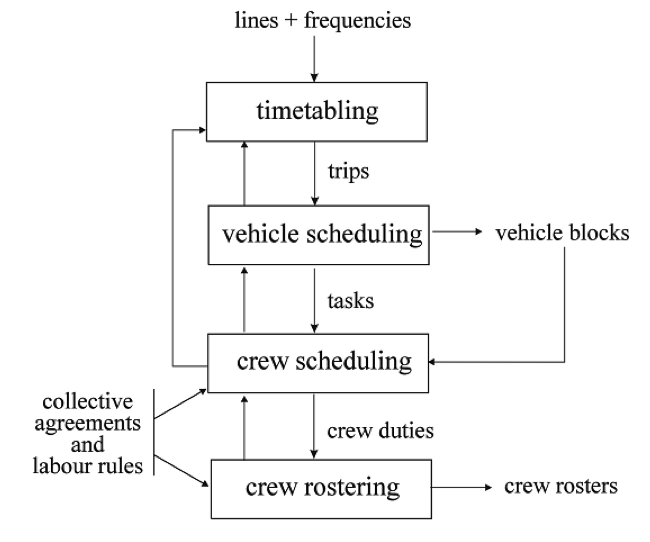
\includegraphics {genericSchedulingProcess}
\caption [Scheduling Process of a Public Transport Company] {Scheduling Process of a Public Transport Company. Source: \cite{Huisman2004}}
\label {image-genericSchedulingProcess}
\end {figure}

Decisions about which routes or lines to operate and how frequently, are inputs for the operational planning process. They can be either given by the marketing department of the company or determined by (local, regional or national) authorities. Furthermore, the travel times between various points on the route are assumed to be known. Based on the lines and frequencies, timetables are determined resulting in trips with corresponding start and end locations and times.

The second planning process is vehicle scheduling which consists of assigning vehicles to trips, resulting in a schedule for each vehicle. The vehicles, which are not in use for some time, are parked in a depot. A schedule for a vehicle is split into several vehicle blocks, where a new vehicle block starts at each departure from the depot. On such a block a sequence of tasks can be defined, where each task needs to be assigned to a working period for one crew (a duty) in the crew scheduling process. The feasibility of a duty is dependent on a set of collective agreements and labor rules that refer to sufficient rest time etcetera. Crew scheduling is short term crew planning (one day), i.e. assigning crew duties to tasks on each specific day, while the crew rostering process is long term crew planning (e.g. half a year) for constructing rosters from the crew duties \cite{Huisman2004}.

\subsection{Timetabling}

\paragraph{ } Timetabling is the process of determining how frequently buses must operate on routes based on passenger demand and the operational plan of the respective authority and generating corresponding start and end locations and times of trips, based on these frequencies. Furthermore travel times between various points in routes, lengths of routes are assumed to be known \cite{Huisman2004}.

The main consideration in the process of timetabling is the output of headways, or the time between consecutive buses. Currently, average optimal headways are calculated in Sri Lanka and used in the scheduling process. An explanation of the current process as it operates in Sri Lanka has been given in the previous chapter.

Let us take a look at previous research done into this area. \cite{Newell1971} provides the basic dispatching policy for a transportation route. This work has been the basis for many future work including \cite{Kumarage2007}'s research paper on formulating an optimal bus dispatching policy under variable demand over time and route length as is the case in Sri Lanka. The paper considered a method that was an extension to \cite{Newell1971}'s Optimal Dispatching Policy to determine a fleet size and dispatching rate based on both the operator's cost and user's cost including the disutility of standing, in order to arrive at a global cost optimum.

\subsubsection{Stochastic model for bus dispatching}

\paragraph{} Previous researchers have proposed a stochastic model for bus dispatching that uses a linear programming model so that it is solvable easily and can be used for other modes of mass transit as well \cite{Riano2004}. A feature of this model is that it should be applied to modes of mass transit where the frequency is high enough so that users do not need to know the schedule in advance (such as the one in Sri Lanka) The solution technique is based on a novel Transient Little Law.

\subsubsection{Adaptive control scheme to mitigate bus bunching}

\paragraph{} Alternatively, an adaptive control scheme to mitigate the problem of bus bunching in a public bus transport system can also be used \cite{Daganzo2008}. This is a problem closely related to timetabling and scheduling and thus has been included in this Literature Review. Bus schedules cannot be easily maintained on busy lines with short headways. Experience and research observation shows that buses offering this type of service usually arrive irregularly at their stops, often in bunches. Although authorities build slack into their schedules to alleviate this problem, if necessary holding buses at control points to stay on schedule, their attempts often fail because practical amounts of slack cannot prevent large localized disruptions from spreading system-wide \cite{Daganzo2008}.

The proposed scheme dynamically determines bus holding times at a route’s control points based on real-time headway information. The method requires less slack than the conventional, schedule-based approach to produce headways within a given tolerance. This allows buses to travel faster, reducing in-vehicle passenger delay and increasing bus productivity. One disadvantage of this method when thinking in terms of a Sri Lankan context is that it requires real-time information which cannot be obtained currently in the Bus Transport System in Colombo.

\subsubsection{Dynamic holding strategies to improve schedule reliability}

Dynamic holding strategies can also be used to improve schedule reliability of a public bus transport system \cite{Xuan2011}. These use the current state of all buses, as well as a virtual schedule. The virtual schedule is introduced whether the system is run with a published schedule or not. Through previous research, it was found that through a dynamic holding strategy buses can both closely adhere to the schedule and maintain regular headways without too much slack. This in turn improves schedule reliability and commercial speed of the buses.

\subsubsection{Derivation of vehicle departure times with even average passenger loads}

Another method of looking at the problem of dispatching buses is to use a methodology framework with developed algorithms for the derivation of vehicle departure times (timetable) with either even headways or even average passenger loads \cite{Ceder2009}. The latter would be ideal for a situation like in Sri Lanka where overcrowding is a major complaint among the commuters.

\subsubsection{Optimizing mathematical model of bus departure interval}

An optimizing mathematical model of bus departure interval could also be used to dispatch buses efficiently. By optimizing a mathematical model of bus departure interval, which takes crowding cost of passengers into account, including passengers’ on-the-bus time cost, passengers’ crowding cost and bus company cost an optimum bus dispatching interval can be calculated. A genetic algorithm could be used to solve the calculation. Research has shown that reasonable bus departure intervals can be obtained quickly by this method \cite{Qian2013}.

\subsubsection{Novel dispatching methodologies}

Novel transit operating strategies can also be thought up to improve the efficiency of a bus transportation service. Service vehicles could operate in pairs with the lead vehicle providing an all-stop local service and the following vehicle being allowed to skip some stops as an express service to address the bus dispatching and timetabling problem. Research has shown that the underlying scheduling problem could be formulated as a nonlinear integer programming problem with the objective of minimizing the total costs for both operators and passengers and solved \cite{Fu2003}. This could possibly be adapted into the Sri Lankan context as a viable alternative to the current scheduling methodology.

Finally, headway optimization and scheduling combination of Bus Rapid Transit (BRT) vehicles could be used and applied to a Sri Lankan context to possibly improve the timetabling and dispatching of buses. Previous research points to a model that minimizes passengers' travel costs and vehicles' operation cost, and constraints included passenger volume, time, and frequency \cite{Sun2008}. The scheduling combination is composed of Normal, Zone, and Express scheduling. The model was solved by a genetic algorithm of variable-length coding. The result of the numerical case showed that the optimization results can save 69.92\% of the cost. A sensitivity analysis that was carried out showed that, under higher traffic volume or lower speed, the travel cost can be reduced through reasonable scheduling combination. Therefore, the method is scientifically proven and is feasible. A similar scheduling method of using Normal, Zone and Express Scheduling could possibly be implemented in Sri Lanka.

\subsection{Vehicle Scheduling}

\paragraph{ } Vehicle scheduling is defined as the process of assigning vehicles, to a set of predetermined trips, with fixed starting and ending times, while minimizing capital and operational costs. According to \cite{Freling2003}, the main objective of this step in the Scheduling Process is keeping the operational and capital costs of vehicles to a minimum.

The Vehicle Scheduling problem can be thought of through two perspectives. They are the Single-Depot Vehicle Scheduling Problem (SDVSP) and the Multiple-Depot Vehicle Scheduling Problem (MDVSP). As noticeable by their names, the difference is the number of depots that each Vehicle is assigned to. In the former, a given vehicle is assigned to a single depot while the latter situation assumes that a given vehicle is assigned to multiple depots. The SDVSP further assumes that all vehicles are identical and there are no time constraints \cite{Huisman2004}. Of these 2 approaches, only the SDVSP applies to the Sri Lankan context as each bus (and its crew) is issued a permit to ply on one route. Therefore, \cite{Freling2003} defines the Single-Depot Vehicle Scheduling Problem as follows.

“Given a depot at location \textit{d} and \textit{n} trips from locations \textit{b}$_i$ to \textit{e}$_i$, with corresponding fixed times \textit{bt}$_i$ and \textit{et}$_i$ (\textit{i}=1,...,\textit{n}),  and  given  the  travelling  times  between  all  pairs (\textit{d}, \textit{b}$_i$), (\textit{b}$_i$, \textit{e}$_i$), (\textit{e}$_i$, \textit{b}$_j$) and (\textit{e}$_i$, \textit{d}), find a feasible \textit{minimum cost} schedule for the vehicles, such that all trips are covered by a vehicle. Each trip has to be entirely serviced by one vehicle and trips serviced by the same vehicle are linked by \textit{deadheading trips} (\textit{dh}-trips).  These are trips without serving passengers (pairs (\textit{d}, \textit{b}$_i$), (\textit{e}$_i$, \textit{b}$_j$) and (\textit{e}$_i$, \textit{d})), consisting of travel time (vehicle deadheading) and/or \textit{idle time} (vehicle waiting time). A schedule for a vehicle is composed of vehicle \textit{blocks}, where each block is a departure from the depot, the service of a sequence of trips and the return to the depot. The cost function is a combination of vehicle capital (fixed) and/or operational (variable) cost. The capital cost is often such that the number of vehicles will be minimized, while the operational cost is often a combination of vehicle travel and idle time”.

In the Multiple-Depot Vehicle Scheduling Problem (MDVSP), buses are dispatched from several depots and total vehicles costs have to be minimized subject to the following constraints \cite{Huisman2004}

\begin {itemize}
\item Every vehicle is associated with a single depot; 
\item Every trip has to be assigned to exactly one vehicle; 
\item Some trips have to be assigned to vehicles from a certain subset of depots.
\end {itemize}

\subsection {Crew Scheduling}

\paragraph{ } The next step in the traditional scheduling process is the Crew Scheduling.  The problem is defined as follows: “The Crew Scheduling Problem (CSP) deals with assigning tasks to duties such that each task is performed; each duty is feasible with respect to a set of working rules and the total costs of the duties are minimized”. 

According to \cite{Huisman2004}, the only requirement with relation to the feasibility of a duty is its length or the working time in that duty, respectively. In most literature, the CSP is formulated as a set partitioning or covering problem and solved with a column generation approach.

\subsection {Integrated Vehicle and Crew Scheduling}

\paragraph{ } As mentioned previously in this chapter, the industry has begun using Integrated Vehicle and Crew Scheduling in recent times. This is due to logical as well as financial reasons. The airline industry uses this methodology as a crew has to be scheduled along with an airline trip for obvious reasons.

The Integrated Vehicle and Crew Scheduling Problem (Integrated VCSP or IVCSP) is analyzed by \cite{Huisman2004}. Accordingly, the Integrated Vehicle and Crew Scheduling Problem is defined as follows. “Given a set of service requirements or trips within a fixed planning horizon, find a minimum cost schedule for the vehicles and the crews, such that both the vehicle and the crew schedules are feasible and mutually compatible. Each trip has fixed starting and ending times, and the travelling times between all pairs of locations are known. A vehicle schedule is feasible if (1) each trip is assigned to a vehicle, and (2) each vehicle performs a feasible sequence of trips, where a sequence of trips is feasible if it is feasible for a vehicle to execute each pair of consecutive trips in the sequence”.

The author provides a very comprehensive look into the problem and presents a methodology to solve integrations of both the SDVSP and the MDVSP. The Integrated VCSP is also discussed by \cite{Freling2000} and \cite{Wren1997}.

\subsection {Crew Rostering}

The Crew Rostering Problem (CRP) aims at determining an optimal sequencing of a given set of duties into rosters satisfying operational constraints deriving from union contracts and company regulations. In the public bus transport industry, the roster is used to evenly distribute the workload among the crew \cite{Caprara1995}. Further studies were done by \cite{Kharraziha2003} and \cite{Tian2012}. The Integrated Crew Rostering Problem was examined in depth by \cite{Valdes2010} and \cite{Xie2012}.

This literature review looked at the different steps involved in the bus scheduling process. It also reviewed the literature related to each step. This literature is what will act as reference material as we attempt to present a new model of scheduling buses. The next chapter will detail the research methodology and the proposed model for scheduling buses in the Western Province.



\section{Loitering of Buses at Bus Stops}
\label{loitering}

\paragraph{} Loitering refers to the time the bus lingers at the bus stop waiting for more passengers after the initial group of passengers have alighted and boarded the bus. The time taken for commuters to get on and off the bus is not considered under the Loiter Time. A common complaint by commuters which is backed by research observations is that buses idle at the bus stop usually until the next bus arrives after dropping off the passengers and allowing others to get in. This leads to the people who are already in the bus waiting idly at the bus stop in a crowded bus senselessly. This action also picks up the passengers that are meant to go in the later bus which leads to the later bus not having enough passengers to cover their costs and thereby they too loiter at the bus stop. This occurs continuously resulting in the commuters being kept waiting in the bus at the bus stop for no reason. 

Loitering is a major issue with the Private Bus Service and frequent complaints are made by commuters regarding it. It is detrimental to the proper dispatching of buses as it delays the commuters and makes it difficult for the schedulers to draw up correct timetables \cite{Mahesh2013a, Theja2013a, Mahesh2013b, Navaratne2013a, Navaratne2013b}.



\section{Automated Data Gathering}

\paragraph{ } While an automatic data gathering system would be immensely helpful to the scheduling unit of the \acrshort{wp} \acrshort{rpta}, there is no such system in place currently. Such a system would aid in formulating proper timetables as well as monitoring and regulating the timetables and the buses for their adherence to said timetables. Proper and accurate data is very difficult to gather at the moment as all data gathering is done manually. This involves a huge amount of man-hours of work not forgetting the fact that the sample gathered is assumed to be representative of the whole system which might not always be the case.

\subsection{Automated Data Collection Systems}

Automatic Data Collection Systems (\acrshort{adcs}) include provisions for Automatic Vehicle Location (AVL) data, Automatic Passenger Count (APC) data as well as the integration of an Automatic Fare Collection (AFC) System. Please refer to Figure~\ref{image-ADCS}. This would allow the schedulers to formulate much more accurate timetables taking into account the Passenger Demands (Load Factors) of the various buses at the various stops during various times of day. An Origin-Destination Matrix could also be obtained by analyzing this data to determine which segments of routes are most frequently used and therefore are more likely to be congested \cite{Wilson2008}.

\begin {figure} [H]
\centering

\includegraphics[scale=0.6]{ADCS}
\caption [An Automatic Data Collection System] {An Automatic Data Collection System}
\label {image-ADCS}
\end {figure}

An implementation of an Automatic Data Collection System (ADCS) could ultimately lead to the creation of Dynamic Timetables. This means that the buses could be scheduled using real-time passenger demand data as well as traffic information and thus would better suit the commuters. However, the current system is to do the scheduling process manually in a strictly procedural fashion.

An ADCS has been proposed in the past but has been shot down and discouraged by the bus owners and operators. The main reason that they point out is that the system is too costly for them to implement and it brings no additional value to them. This is a misguided notion by the owners and operators as the system could benefit them immensely in the long run. Revenue leakage, which is one of the main grievances given by bus owners, could be curbed through an implementation of an Automatic Fare Collection (AFC) system. Furthermore, it would bring about a sense of accountability and transparency in the payment of fares of private buses. It would be a cost in the short-term, but considering the long-term benefits, the owners/operators should consider it an investment to make the system and service future-proof.

Furthermore, an Automatic Vehicle Location (AVL) system would allow commuters to know exactly where and when the next bus will be arriving providing more information and flexibility. Automatic Passenger Counting (APC) would give the schedulers enough information to ensure that timetables are working correctly and buses are dispatched to account for higher or lower passenger demand. The schedulers could also audit their timetables more frequently to ensure that schedules are kept current. It would also allow route monitors to ascertain if the owners/operators are overcrowding the buses causing discomfort to passengers. An Automatic Fare Collection (AFC) system would also bring great comfort to commuters who consistently complain about being overcharged or not receiving the proper balance money back from the conductor. An An Automatic Fare Collection (AFC) system would also greatly benefit the owners/operators because they could monitor and audit their income correctly and put paid to the revenue leakage that occurs consistently (according to the owners) \cite{Wilson2008, Wilson2009, Wilson2012, Fijalkowski2010}.

\subsection{Automatic Vehicle Location (AVL)}

\paragraph{ } Vehicle Location data could be obtained through several methods. One of the main and most feasible methods would be to fix a GPS-based tracker on to the bus and monitoring its movement through a mapping software. This method, however, has a fairly large startup cost which has discouraged the stakeholders in the past. Alternatively, this could be achieved by crowdsourcing the Vehicle Location data through a mobile app. Automatic Vehicle Location (AVL) Data is very important as it reflects the current location of a bus and can be used to predict journey times and availability of buses for the commuters. A system could be built that uses AVL data to notify commuters of the current bus, the bus that is due to arrive next etc. This data is also very important in the scheduling stage of transport planning and could be used to formulate more efficient and effective timetables \cite{Wilson2009}.

\subsection{Automatic Passenger Counting (APC)}

\paragraph{ } Automatic Passenger Counting (APC) is important in order to gauge the passenger demand or load factors in the buses. This data could be used to draw up origin-destination matrices in order to identify which segments of routes are most congested and which routes are not very congested at all. This all helps in the planning and dispatching of buses which eventually lead to a better schedule and a better service.

The APC data could be obtained from an Automated Fare Collection (AFC) System such as a contactless smart card payment method. The implementation of both could potentially be very useful for the commuters and owners/operators alike \cite{Wilson2009, Silva2010}.

\subsection{Automatic Fare Collection (AFC)}

\paragraph{ } The implementation of an Automatic Fare Collection system has been in the works for some time and discussions with industry experts have revealed that a working system is available. However it is not being implemented as the government still has some regulatory and other issues to sort out first. The system involves a Prepaid Smart Card system where the Smart Card could be used for cashless payment of bus fares. Commuters could also recharge their cards when the stored value in the cards runs low (akin to reloading a prepaid mobile phone). This is just one of the methods that could be used to implement an automated fare collection system \cite{Wilson2009, Silva2010}.

\subsection{\acrshort{nfc} in public transportation}

\paragraph{} As its popularity grows, \acrshort{nfc} or Near-Field Communication has garnered the attention of public transport systems around the world. It allows a user to use everyday devices (such as a mobile phone or an \acrshort{atm} card etc.) as a transaction medium. This could lead to enabling payment of bus fares with a mobile phone which is a very innovative and highly lucrative area to look into. It would bring comfort to passengers and allow owners/operators to receive the payment directly from the commuters. Therefore, the potential market and it's applications is vast. However, Sri Lanka does not have any such systems or parties interested in a system like this which is unfortunate. One could argue that before going to such technologically advanced lengths, the authorities should focus on a smaller system and implement one which is more appropriate to the Sri Lankan context which is a fair argument. The problem is that currently \textit{no system at all} exists, which is not a good situation for the private bus service and the country \cite{Silva2010, Sinha2012}.

\subsection{Automatic Data Collection in the Inter-Provincial Service} 

\paragraph{ } An Automatic Data Collection System is in place at the moment in the Inter-Provincial buses. The National Transport Commission (NTC) has taken steps to implement a system to track the location of the buses via a GPS tracking device fixed onto them. However, out of the 3500+ buses in operation in the Inter-Provincial service, only around 700 have been fixed with the device. Information obtained from the NTC states that a further 1000 buses will be equipped with the device within this year.

Currently, it only tracks the location and the speed of the bus. The system they have implemented consists of a device which is fixed on to the vehicle. This device tracks the location of the bus via GPS and relays the data back to the NTC servers via a GPRS connection. The device also contains an accelerometer to measure the speed of the vehicle. This allows the NTC to monitor the buses for possible speeding violations and reckless driving. Monitoring is done through a control center at the NTC head office in Narahenpita which is manned 24 hours a day. Apart from monitoring the buses, they provide information to the passengers and record complaints regarding errant bus operators.

Owners/operators can also choose to have a still camera fixed onto the bus as well. This is compulsory for Luxury buses and it allows the NTC monitor overcrowding of the buses. When a complaint is made to the NTC hotline, the personnel at the NTC control center can activate the camera and take a picture to decide if the bus is overcrowded or not. They can then instigate punishment proceedings for the bus involved.

The device costs around 45,000 rupees with the government subsidizing the cost. Eventually, the owners/operators have to pay only around 10,000 rupees. The objective of the NTC is to eventually have all the inter-provincial buses fitted with the device. This would allow the data to be collected automatically and that data would be used for the scheduling process and the formulation of timetables for the service (Source: Interviews with personnel at the NTC).

As mentioned previously, the NTC has implemented a GPS-based Vehicle Tracking system in the Inter-Provincial Bus Transport Service as an Automated Data Collection System. However, it only collects the Vehicle Location data. The Passenger Counts data is not collected automatically and there is no system in place to do so. However, the Inter-Provincial Bus Service is more developed than the Intra-Provincial Service in the Western Province as the NTC has made it compulsory for Inter-Provincial buses to have Electronic Ticketing Machines (ETM). This means that at least the passenger counts data \textit{is} recorded. The data that is saved in the Ticketing Machines could be accessed later and the data be obtained for scheduling purposes.

\section{Decision Support Systems}
\label {section-DSS}

\paragraph{ } Decision Support Systems are defined as a set of related computer programs and the data required to assist with analysis and decision-making within an organization. They are purposely developed to improve decision making of non-structured management problems. Decision Support Systems utilize data, provide an easy-to-use interface, and allow for the decision maker’s own insights hence being interactive, flexible, and adaptable computer-based information systems \cite{Turban2005}. 

Having said that, the term DSS in itself is difficult to define with academics and users differing in their opinion in terms of its preferred use. While academics have perceived DSS as a tool to support the decision making process, DSS users see DSS as a tool to facilitate organizational processes \cite{Keen1980}.

\subsection{History of Decision Support Systems}

\paragraph{ } The concept of a Decision Support System has been around since the 1950's but only recently has it increased in popularity and adoption in the industry. With the improvement in technology, the research into DSS's has also increased. The abstract concept of a system that aids in the decision-making process has its roots in the late 1950's and early 1960's through research done at the Carnegie Institute of Technology. This later grew into information systems research through work done at the Massachusetts Institute of Technology in the 1960's. DSS's started to become a research topic of its own in the mid-1970's with more and more research following through the mid to late 1980's \cite{Keen1980, Power2003}.

\subsection{Categories of Decision Support Systems}

\paragraph{} There are 5 main categories of DSS's which are \cite{Power2003},

\begin {itemize}
\item \textbf{Communication-driven DSS} is a type of DSS that emphasizes communications, collaboration and shared decision-making support. A simple bulletin board or threaded email is the most elementary level of functionality. The comp.groupware FAQ defines groupware as "software and hardware for shared interactive environments" intended to support and augment group activity. Groupware is a subset of a broader concept called Collaborative Computing. Communications-Driven DSS enable two or more people to communicate with each other, share information and co-ordinate their activities. Group Decision Support Systems or GDSS is a hybrid type of DSS that allows multiple users to work collaboratively in groupwork using various software tools. Examples of group support tools are: audio conferencing, bulletin boards and web-conferencing, document sharing, electronic mail, computer supported face-to-face meeting software, and interactive video.; 
\item \textbf{Data-driven DSS} is a type of DSS that emphasizes access to and manipulation of a time-series of internal company data and sometimes external data. Simple file systems accessed by query and retrieval tools provide the most elementary level of functionality. Data warehouse systems that allow the manipulation of data by computerized tools tailored to a specific task and setting or by more general tools and operators provide additional functionality. Data-driven DSS with On-line Analytical Processing (OLAP) provides the highest level of functionality and decision support that is linked to analysis of large collections of historical data. Executive Information Systems (EIS) and Geographic Information Systems (GIS) are special purpose Data-Driven DSS.;
\item \textbf{Document-driven DSS} is a relatively new field in Decision Support. A document driven DSS is focused on the retrieval and management of unstructured documents. Documents can take many forms, but can be broken down into three categories: Oral, written, and video. Examples of oral documents are conversations that are transcribed; video can be news clips, or television commercials; written documents can be written reports, catalogs, letters from customers, memos, and even e-mail.;
\item \textbf{Knowledge-driven DSS} can suggest or recommend actions to managers. These DSS are person-computer systems with specialized problem-solving expertise. The "expertise" consists of knowledge about a particular domain, understanding of problems within that domain, and "skill" at solving some of these problems.;
\item \textbf{Model-driven DSS} emphasize access to and manipulation of a model, for example, statistical, financial, optimization and/or simulation models. Simple statistical and analytical tools provide the most elementary level of functionality. Some OLAP systems that allow complex analysis of data may be classified as hybrid DSS systems providing both modeling and data retrieval and data summarization functionality. In general, model-driven DSS use complex financial, simulation, optimization or multi-criteria models to provide decision support. Model-driven DSS use data and parameters provided by decision makers to aid decision makers in analyzing a situation, but they are not usually data intensive, which means very large databases are usually not needed for a model-driven DSS.;
\end {itemize}

 4 main characteristics of \acrshort{dss}'s can be identified \cite{Power2003}.

\begin {enumerate}
\item Inputs - these are what is used by the DSS analysis.;
\item User knowledge and expertise - this allows the system to decide how much it is relied on, and exactly what inputs must be analyzed with or without the user.;
\item Outputs - this is used so that the user of the system can analyze the data and potentially make a decision based on the information presented.;
\item Decision Making - this is the ultimate goal of the User who utilizes the DSS. The goal of the system is to aid the User in their decision-making process.;
\end {enumerate}

This chapter provided the theoretical basis for this research. It included an explanation of what a typical planning process of a public transport system entails and also provided a description of how Automated Data Collection Systems factor into the planning process. The chapter ended with a look at what Decision Support Systems are, it's categories, a brief look at its history and its uses. A justification of how Decision Support Systems relate to the problem at hand was given previously in this document. The next chapter will detail the research methodology that was followed during this project. 


